% \begin{frame}{Virtual Analog Modelling}
%     Creating a digital emulation of a classic analog audio effects.
%     \vspace{1ex}
%     \begin{itemize}
%         \itemsep0em
%         \item Provide access to effects that are old or rare.
%         \item Lower cost.
%         \item Convenience.
%         \item Improved understanding.
%     \end{itemize}
% \end{frame}

% \begin{frame}{Klon Centaur}
%     Guitar pedal made by Bill Finnegan (MIT) from 1994-2000
%     \vspace{1ex}
%     \begin{figure}
%         \centering
%         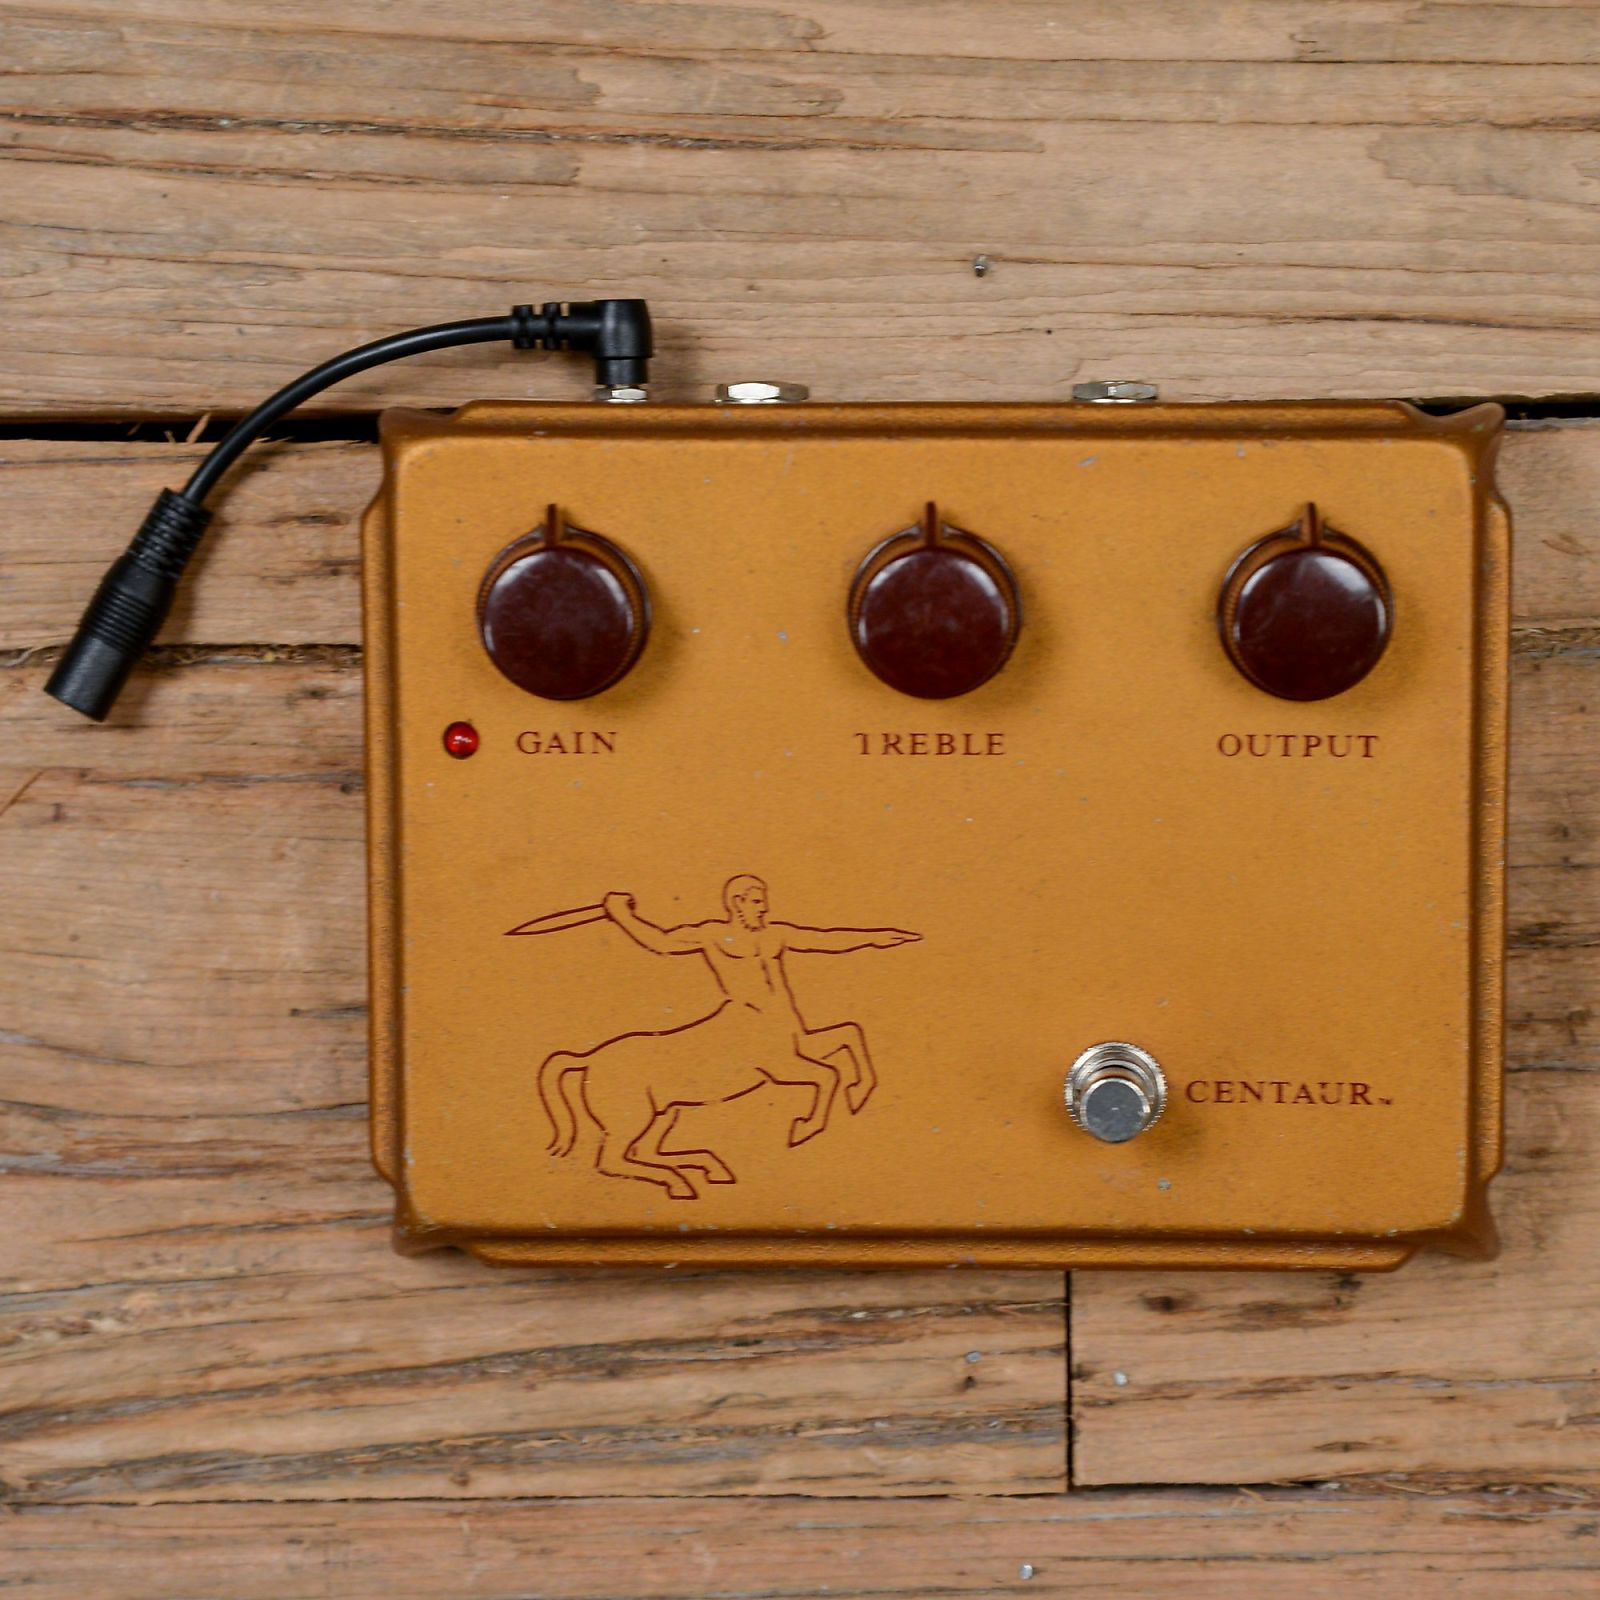
\includegraphics[height=2.5in]{../Paper/Figures/KlonCentaur.jpg}
%     \end{figure}
% \end{frame}

% \begin{frame}{Klon Centaur Circuit Schematic}
%     \begin{figure}
%         \centering
%         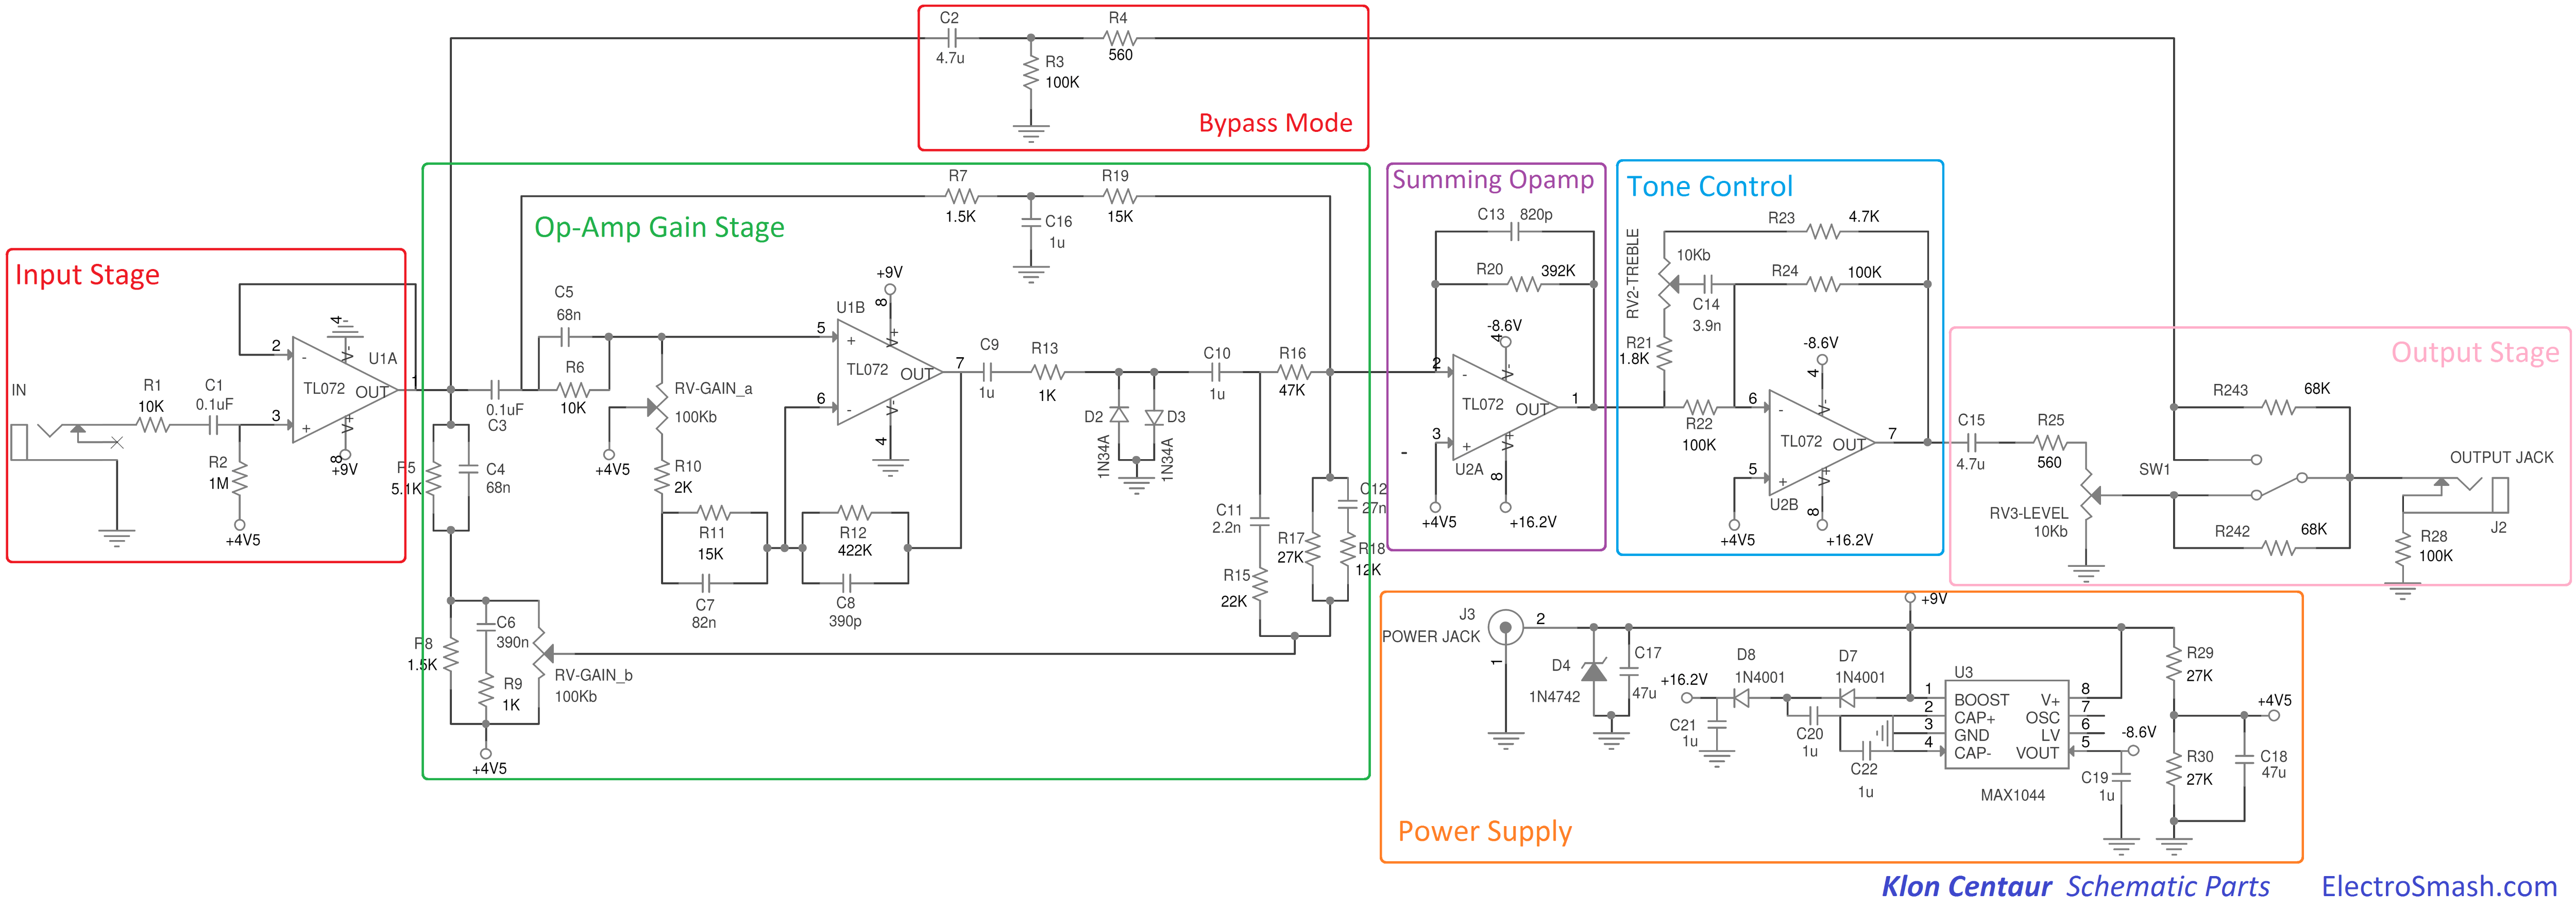
\includegraphics[width=5.5in]{../Paper/Figures/FullCircuit.png}
%     \end{figure}
% \end{frame}

% \begin{frame}
%     \begin{centering}
%         \vskip5ex plus 1filll
%         {\usebeamerfont{title page title}\usebeamercolor[fg]{title page} Traditional Circuit Modelling\\[1.5ex]}
%         \vskip0pt plus 1filll
%     \end{centering}
% \end{frame}

% \begin{frame}{Nodal Analysis\footcite{pasp,Maby}}
%     \begin{figure}
%         \centering
%         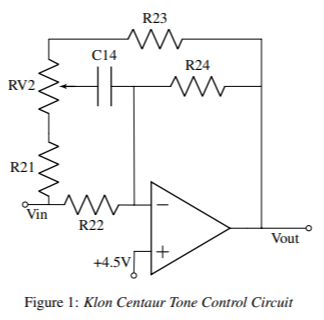
\includegraphics[height=2.5in]{Figures/ToneControl.png}
%     \end{figure}
% \end{frame}

% \begin{frame}{Nodal Analysis}
%     Laplace domain transfer function
%     \begin{equation}
%         \frac{V_{out}(s)}{V_{in}(s)} = {\scriptscriptstyle \frac{C_{14}\left(\frac{1}{R_{22}} + \frac{1}{R_{21} + R_{v2b}}\right)s
%         + \frac{1}{R_{22}}\left(\frac{1}{R_{21} + R_{v2b}} + \frac{1}{R_{23} + R_{v2a}}\right)}{
%           C_{14}\left(\frac{1}{R_{23} + R_{v2a}} + \frac{1}{R_{24}}\right)s
%         + \frac{-1}{R_{24}}\left(\frac{1}{R_{21} + R_{v2b}} + \frac{1}{R_{23} + R_{v2a}}\right)}}
%     \end{equation}
%     %
%     Bilinear transform (or other conformal map)
%     \begin{equation}
%         s \leftarrow \frac{2}{T} \frac{1 - z^{-1}}{1 + z^{-1}}
%     \end{equation}
% \end{frame}

% \begin{frame}{Nodal Analysis}
%     \begin{figure}
%         \centering
%         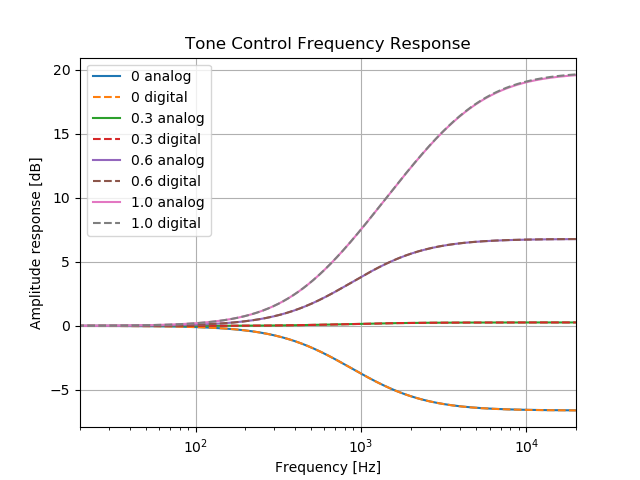
\includegraphics[height=2.75in]{../Paper/Figures/ToneFreq.png}
%     \end{figure}
% \end{frame}

% \begin{frame}{Wave Digital Filters (WDFs)\footcite{Fettweis,KurtThesis}}
%     \begin{figure}
%         \centering
%         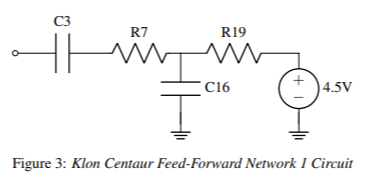
\includegraphics[height=2.0in]{Figures/FF1.png}
%     \end{figure}
% \end{frame}

% \begin{frame}{Wave Digital Filters (WDFs)}
%     \begin{columns}
%         \begin{column}{0.45\linewidth}
%             \hspace{-1ex}
%             \begin{itemize}
%                 \item Use wave variables instead of voltage/current.
%                 \item Port resistance free parameter.
%                 \item Discretize each circuit element separately.
%             \end{itemize}
%         \end{column}
%         \begin{column}{0.55\linewidth}
%             \begin{figure}
%                 \centering
%                 \begin{tikzpicture}[node distance=1.25cm]
%                     \tikzset{
%                         arrow/.style = {thick,->,>=stealth}
%                     }
%                     \node (Vin) {$V_{in}$};
%                     \node (S1)  [right of=Vin] {$\mathcal{S}_1$};
%                     \node (C3)  [right of=S1, below of=S1, yshift= 0.5cm] {$C_3$};
%                     \node (S2)  [right of=S1, above of=S1, yshift=-0.5cm] {$\mathcal{S}_2$};
%                     \node (R7)  [right of=S2, above of=S2, yshift=-0.5cm] {$R_7$};
%                     \node (P1)  [right of=S2, below of=S2, yshift= 0.5cm] {$\mathcal{P}_1$};
%                     \node (C16) [right of=P1, below of=P1, yshift= 0.5cm] {$C_{16}$};
%                     \node (S3)  [right of=P1, above of=P1, yshift=-0.5cm] {$\mathcal{S}_3$};
%                     \node (R19) [right of=S3, above of=S3, yshift=-0.5cm] {$R_{19}$};
%                     \node (V45) [right of=S3, below of=S3, yshift= 0.5cm] {$V_{4.5}$};
            
%                     \draw [arrow] (Vin) -- (S1);
%                     \draw [arrow] (S1) -- (C3);
%                     \draw [arrow] (S1) -- (S2);
%                     \draw [arrow] (S2) -- (R7);
%                     \draw [arrow] (S2) -- (P1);
%                     \draw [arrow] (P1) -- (C16);
%                     \draw [arrow] (P1) -- (S3);
%                     \draw [arrow] (S3) -- (R19);
%                     \draw [arrow] (S3) -- (V45);
%                 \end{tikzpicture}
%                 \caption{\label{fig:wdftree}{\it WDF tree for the Klon Centaur Feed-Forward Network 1 Circuit.
%                 $\mathcal{S}$ and $\mathcal{P}$ nodes refer to series and parallel
%                 adaptors respectively.}}
%             \end{figure}
%         \end{column}
%     \end{columns}
% \end{frame}

% \begin{frame}{Wave Digital Filters (WDFs)}
%     \begin{figure}
%         \centering
%         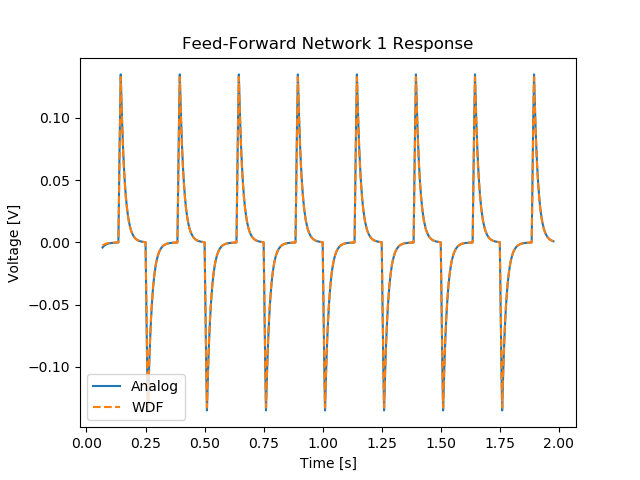
\includegraphics[height=2.75in]{../Paper/Figures/WDFval.png}
%     \end{figure}
% \end{frame}

% \begin{frame}
%     \begin{centering}
%         \vskip5ex plus 1filll
%         {\usebeamerfont{title page title}\usebeamercolor[fg]{title page} Neural Network Circuit Modelling\\[1.5ex]}
%         \vskip0pt plus 1filll
%     \end{centering}
% \end{frame}

% \begin{frame}{Recurrent Neural Network\footcite{VArnn}}
%     \begin{figure}
%         \centering
%         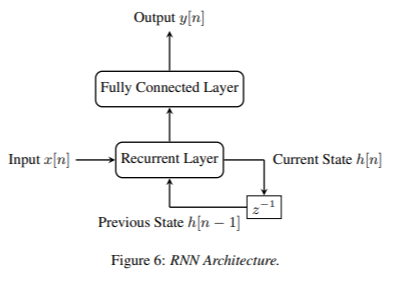
\includegraphics[height=2.5in]{Figures/RNNArch.png}
%     \end{figure}
% \end{frame}

% \begin{frame}{Recurrent Neural Network}
%     Recurrent layer: Gated Recurrent Unit
%     \begin{equation}
%         z[n] = \sigma(W_z x[n] + U_z h[n-1] + b_z)
%     \end{equation}
%     \begin{equation}
%         r[n] = \sigma(W_r x[n] + U_r h[n-1] + b_r)
%     \end{equation}
%     \begin{equation}
%         c[n] = \tanh(W_c x[n] + r[n] \circ U_c h[n-1] + b_c)
%     \end{equation}
%     \begin{equation}
%         h[n] = z[n] \circ h[n-1] + (1 - z[n]) \circ c[n]
%     \end{equation}
% \end{frame}

% \begin{frame}{Recurrent Neural Network}
%     Training Data:
%     \begin{itemize}
%         \itemsep0em
%         \item $\sim 4$ minutes of guitar recordings (direct)
%         \item Split into 0.5 second segments
%         \item 400 training samples, 25 validation samples
%     \end{itemize}
%     \vspace{2ex}
%     Loss Function: Error-to-Signal Ratio
%     \begin{equation}
%         \mathcal{E}_{ESR} = \frac{\sum_{n=0}^{N-1} |y[n] - \hat{y}[n]|^2}{\sum_{n=0}^{N-1} |y[n]|^2}
%     \end{equation}
% \end{frame}

% \begin{frame}{Recurrent Neural Network}
%     Training: 500 epochs, $\sim 8$ hours
%     \begin{figure}
%         \centering
%         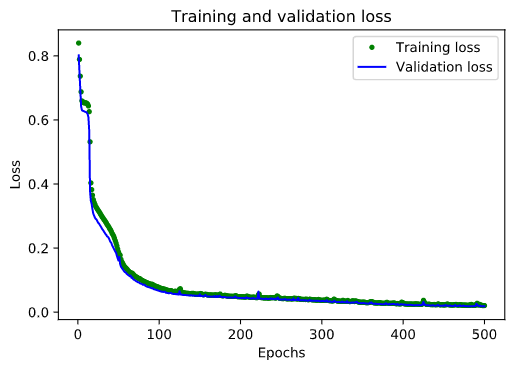
\includegraphics[height=2.5in]{../Paper/Figures/Training.png}
%     \end{figure}
% \end{frame}

% \begin{frame}{Recurrent Neural Network}
%     Training results (time domain)
%     \begin{figure}
%         \centering
%         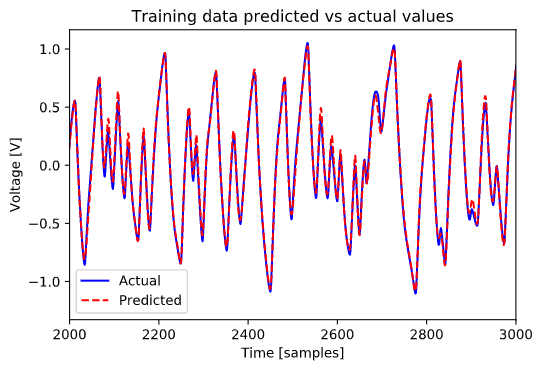
\includegraphics[height=2.5in]{../Paper/Figures/TimeDomain.png}
%     \end{figure}
% \end{frame}

% \begin{frame}{Recurrent Neural Network}
%     Training results (frequency domain)
%     \begin{figure}
%         \centering
%         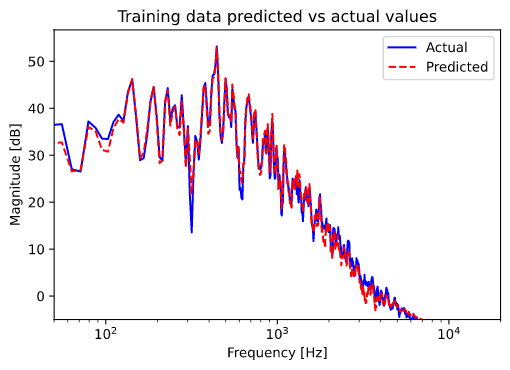
\includegraphics[height=2.5in]{../Paper/Figures/FreqDomain.png}
%     \end{figure}
% \end{frame}

% \begin{frame}
%     \begin{centering}
%         \vskip5ex plus 1filll
%         {\usebeamerfont{title page title}\usebeamercolor[fg]{title page} Real-Time Implementation\\[1.5ex]}
%         \vskip0pt plus 1filll
%     \end{centering}
% \end{frame}

% \begin{frame}{Implementation}
%     \begin{columns}
%         \begin{column}{0.45\linewidth}
%             Non-ML Implementation
%             \begin{itemize}
%                 \item Use a combination nodal analysis, WDFs
%                 \item Control parameters for Treble, Gain, Level
%             \end{itemize}
%         \end{column}
%         \begin{column}{0.55\linewidth}
%             ML Implementation
%             \begin{itemize}
%                 \item RNN model for Gain Stage, nodal analysis elsewhere
%                 \item Fade between models for variable Gain control
%                 \item Custom GRU and Dense layer implementations in C++
%             \end{itemize}
%         \end{column}
%     \end{columns}
% \end{frame}

% \begin{frame}{Implementation}
%     Inference Engine
%     \begin{itemize}
%         \item Why use a custom implentation?
%         \begin{itemize}
%             \item GRU support in TFLite is still experimental
%             \item Real-time audio thread: no locking, no memory allocation
%         \end{itemize}
%         \item Currently using STL functions (\texttt{std::inner\_product})
%         \item Eventually upgrade to Eigen or TFLite
%     \end{itemize}
% \end{frame}

% \begin{frame}{Implementation}
%     Desktop Audio Plugin (JUCE/C++)
%     \begin{figure}
%         \centering
%         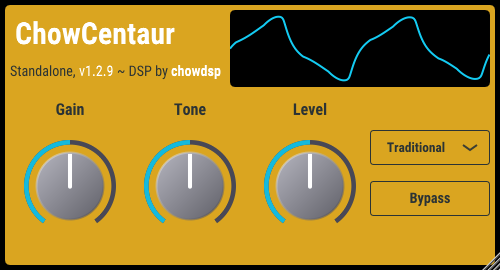
\includegraphics[height=2.5in]{../Paper/Figures/Plugin.png}
%     \end{figure}
% \end{frame}

% \begin{frame}{Implementation}
%     Teensy 4.0, Teensy Audio Shield, Teensy Audio Library
%     \begin{figure}
%         \centering
%         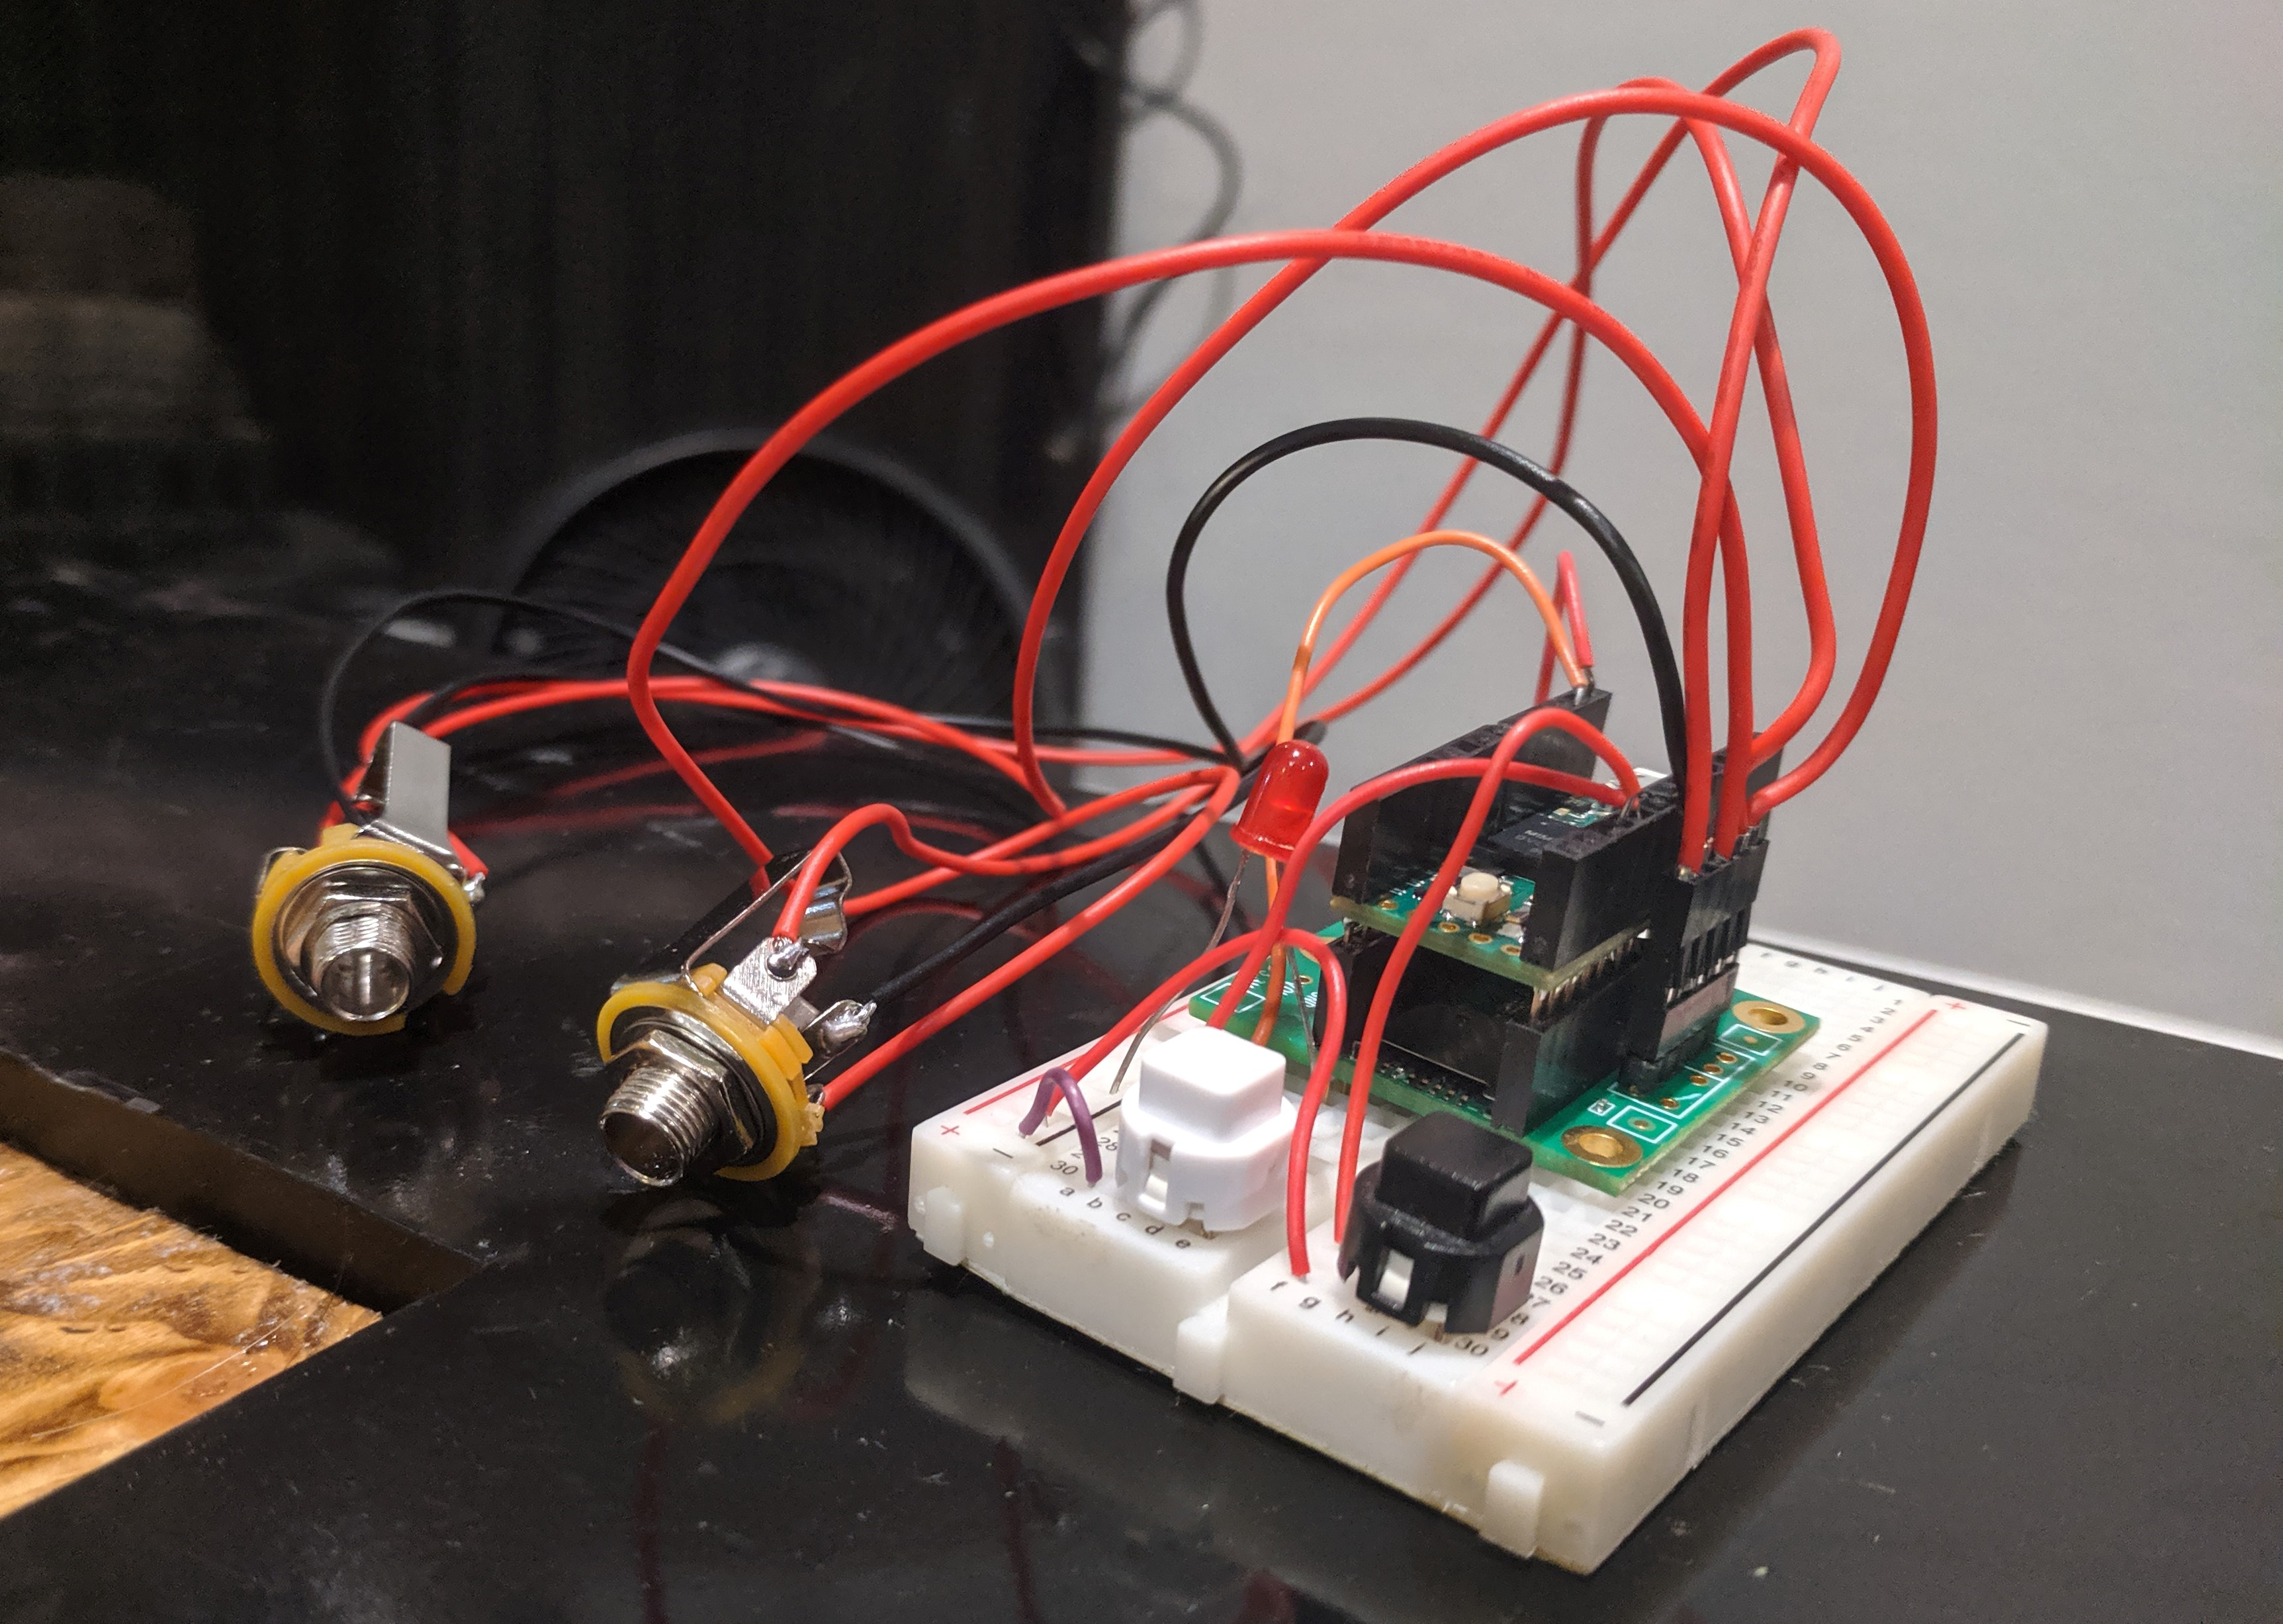
\includegraphics[height=2.5in]{../Paper/Figures/Teensy.jpg}
%     \end{figure}
% \end{frame}

% \begin{frame}{Results: Performance}
%     Compute time per second of audio.
%     \begin{table}[h!]
%         \centering
%          \begin{tabular}{||c | c | c||} 
%          \hline
%          Block Size & NonML Speed & ML Speed \\
%          \hline\hline
%          8    & 0.0723437 & 0.0528792 \\
%          16   & 0.0703079 & 0.0510437 \\
%          32   & 0.0652856 & 0.0511147 \\
%          64   & 0.0662835 & 0.0502434 \\
%          128  & 0.0666593 & 0.0495194 \\
%          256  & 0.0696844 & 0.0480298 \\
%          512  & 0.0669037 & 0.0477946 \\
%          1024 & 0.060816  & 0.0488841 \\
%          2048 & 0.0695175 & 0.0488309 \\
%          4096 & 0.0623839 & 0.0472191 \\
%          \hline
%          \end{tabular}
%     \end{table}
% \end{frame}

% \begin{frame}{Results: Summary}
%     \begin{itemize}
%         \item Subjectively, non-ML and ML models sound very similar.
%         \item ML model has slightly damped high frequency response,
%             (not a big deal on guitar input; more noticeable on other audio).
%         \item ML model is more efficient!
%     \end{itemize}
% \end{frame}

% \begin{frame}
%     \begin{centering}
%         \vskip5ex plus 1filll
%         {\usebeamerfont{title page title}\usebeamercolor[fg]{title page} Live Performance!\\[1.5ex]}
%         \vskip0pt plus 1filll
%     \end{centering}
% \end{frame}
